\documentclass[12pt, a4paper]{scrartcl}
\usepackage[utf8]{inputenc}
\usepackage{graphicx}
\usepackage{amsmath, amsthm, amssymb, textcomp}
\usepackage{setspace}
\usepackage{paralist}
\usepackage{graphicx}
\usepackage{caption}
\graphicspath{{WSK_im/}} %Graphic is in a folder named WSK_im in the currend directory
\usepackage{float}
\usepackage{authblk}
\renewcommand\Authfont{\fontsize{12}{14.4}\selectfont}
\title{Bayesian probability theory - Lesson 1}

\author{Wolfgang von der Linden}
\date{Transscript}

\begin{document}
\setlength{\parindent}{0pt}
\maketitle
\onehalfspacing

Welcome to the first unit in the lecture on Bayesian probability theory. My name is Wolfgang von der Linden and I will enable you to help Captain Bayes and her crew to solve their adventures in probability theory.
The first episode helps us to enter the discussion of Bayesian probability theory.
The aim of this unit is to provide you with the language to describe probabilistic problems, have a first glimpse on the different concepts of probability theory and to enable you to solve elementary problems.\\

Let us start with some definitions that will help us to find a language to formulate problems and solutions.
Problems with uncertain outcome can also be formulated as \textbf{questions}. For example, the "question" may concern a random experiment, as for instance, the random compass. A possible question could be: "In which direction will the compass needle point?". 
Another famous experiment is performed with a dice, where we can ask the question: "How many pips will the dice show at the next throw? 
But the question does not necessarily have to do with random events, like: "What’s for lunch tomorrow?". The uncertainty may just be due to lack of information. It doesn’t even have to have anything to do with future events, which outcome is uncertain for everyone, for instance: “Where is Captain Bayes?” At least Captain Bayes herself will know the answer. All these problems have one aspect in common: the answer is uncertain for whatever reason.
Each "question" has a well-defined set of results which we call \textbf{"outcomes"}. Like the four compass directions: North, East, West, South, or the number of pips on a dice, all the possible dishes for lunch, like "Roast" or "Potatoes", or the whereabouts of Captains Bayes, like in the ship’s galley or on deck and so on ...
We call the total set of possible outcomes the \textbf{sample space} and we denote it by \textbf{$\Omega$}. A question can be associated with a \textbf{random variable} that assigns a real unique number to each outcome. This is especially useful for measurable results, like the number of pips on a dice or the weight of a fish. 
For the directions of the random compass, we can assign an angle. For a question that favors one particular result one can use one for the result itself and zero for all remaining outcomes.\\

Random variables can be \textbf{discrete} or \textbf{continuous}. 
Discrete variables have \textbf{distinct values}, which in many cases are natural numbers, like the pips of the dice. The sample space Omega of a discrete variable is \textbf{countable}. We will focus on discrete variables throughout the first seven units.
Continuous variables, on the other hand have uncountably many values, as for example real number in a certain interval, or the weight of fish, or the angle of a direction, or the time that something happens.
Continuous variables are in some aspects special. Counting of all possible or favorable outcomes is not possible and a different principle of measuring, called \textbf{"measure theory"} has to be used. Interesting phenomena like \textbf{scale invariance} or the \textbf{Bertrand paradox} will await us at the end of this course when continuous variables will be discussed.\\

Now we continue with the formulation of probabilistic "questions" and generalize the result of a random experiment, which so far was called outcome. We want to ask not only the question: "Will the dice show five pips?" but also questions like "Will the dice show an odd number of pips?" which includes the three outcomes "one", "three" and "five".
The generalized result of a random experiment is now formed by a subset of the sample space, which we call an \textbf{event}. Note that we use curly brackets - the set brackets - to indicate a set of elements. There is no order in a set of outcomes in contrast to later discussed tuples of outcomes, where the order is important.
Let us analyze how many events can be formed by the subsets of the sample space. To this end we take a look at the event space, denoted by $\Sigma$, which is the space of all possible subsets of the sample space $\Omega$. We call this also the \textbf{power set of $\Omega$}. 
The smallest event containing no outcome is called the \textbf{empty set} and is never realized. It is therefore also called the \textbf{impossible outcome}.
Events containing only one outcome are called \textbf{elementary events}.
The event that covers the entire sample space is the \textbf{certain event} or \textbf{the one element}. As for the complexity of the questions, there are no restrictions.  We could also consider multiple dice or repeated throws of a single dice. Or we could even combine a dice experiment with the random compass. I leave it up to you to think about the corresponding sample space and the elements of the $\Sigma$ space.\\
\begin{figure}[H]
	\centering
	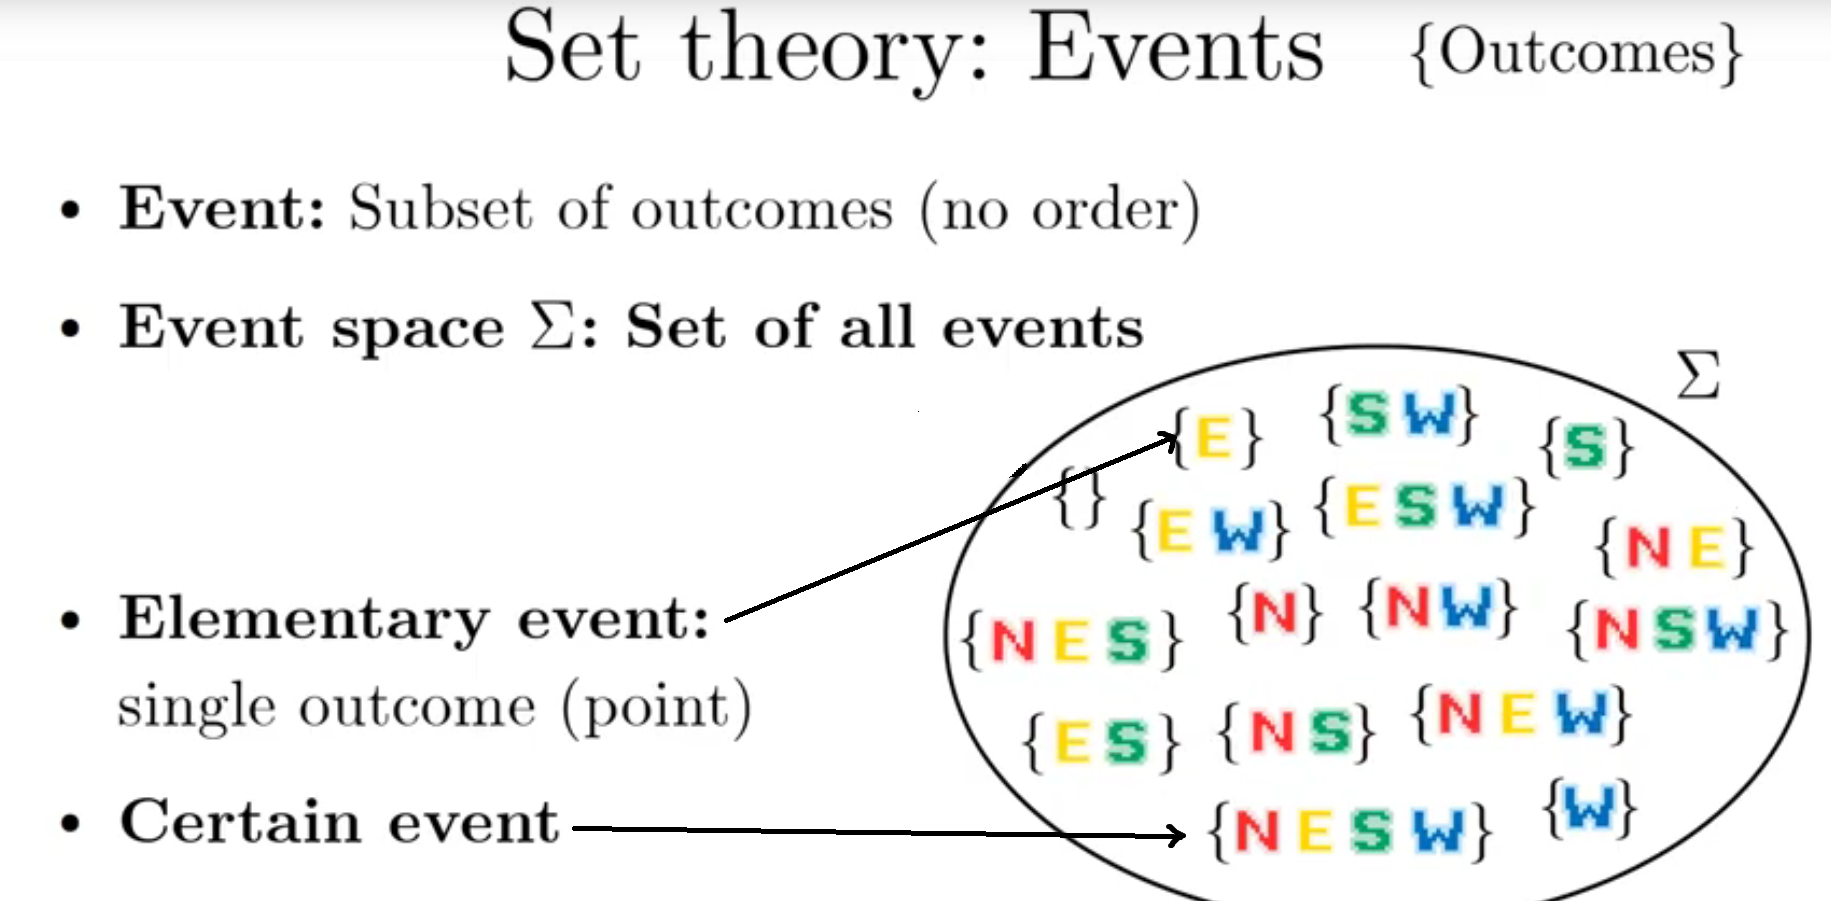
\includegraphics[width=0.75\textwidth]{1_1.png}
\end{figure}
\fbox{\parbox{\linewidth}{\textbf{Question 1.} What are elements of the event space of the combined experiment ``compass and dice''?\\
a) \{(N,1),(E,2), (not S, 2)\}\\
b) \{(N,1), (E,2)\}\\
c) \{\}\\
d) (\{N,1\},\{S,3\})\\
e) \{(N, even number)\}\\
\textbf{Question 2.} Which elements are part of the sample space $\Omega$ of the experiment ``compass and dice''?\\
a) North + South\\
b) 3 + North \\
c) \{S, 1\}
}}
\\

In addition to outcome and event, another term plays a crucial role in probability theory: the \textbf{proposition}. A proposition is a statement that can either be true or false, nothing in between, like the coin will land heads up, or Caesar was a roman. Propositions are particularly obvious in binary experiments. These are experiments with only two outcomes. Such an experiment is called \textbf{Bernoulli trial}. One of the most famous examples is tossing a coin which has the two outcomes heads and tails. 
Every event A can be rephrased as a proposition by stating "The experiment will have event A as its’ result." This proposition can be true or false. The opposite of proposition B can be addressed using the negation operator "NOT" B. We will discuss propositions and their usage in Bayesian Probability Theory in more detail in unit three.
\fbox{\parbox{\linewidth}{\textbf{Question 3.} Which of the following statements is a proposition?\\
a) It was a bad advice.\\
b) Time travel is possible.\\
c) Global warming is man-made.\\
d) Our solar system has only three planets.
}}
\\

Now that we have defined the objects of the probabilistic reasoning it’s time to introduce the notion of \textbf{Probability}. The aim is to assign a number to each event, that quantifies its partial truth. The larger the number, the more likely the event will occur. 
There are some basic assumptions concerning this number, called \textbf{axioms of Kolmogorov}. The first assumption states, that each event is mapped to a real number between zero and one. Zero indicates an impossible event, one that can never happen. A probability one, on the other hand, marks a certain event that will definitely happen, thus called the one event.\\

\fbox{\parbox{\linewidth}{\textbf{Question 3.} What is the certain event of a dice roll?\\
a) The dice will show at least two pips.\\
b) After Sunday follows Monday.\\
c) The dice will show 1,  2, 3, 4, 5, or 6 pips on the top face.
}}
\\

 The zero event and his set will always be mapped to probability zero. It should be noted that there can be more events that have a zero probability. The one event is the set of all possible outcomes, or rather, the entire sample space and it has the probability one. An example for a certain event is "The dice will show any number of pips. Anything between one and six.” 
\begin{figure}[H]
	\centering
	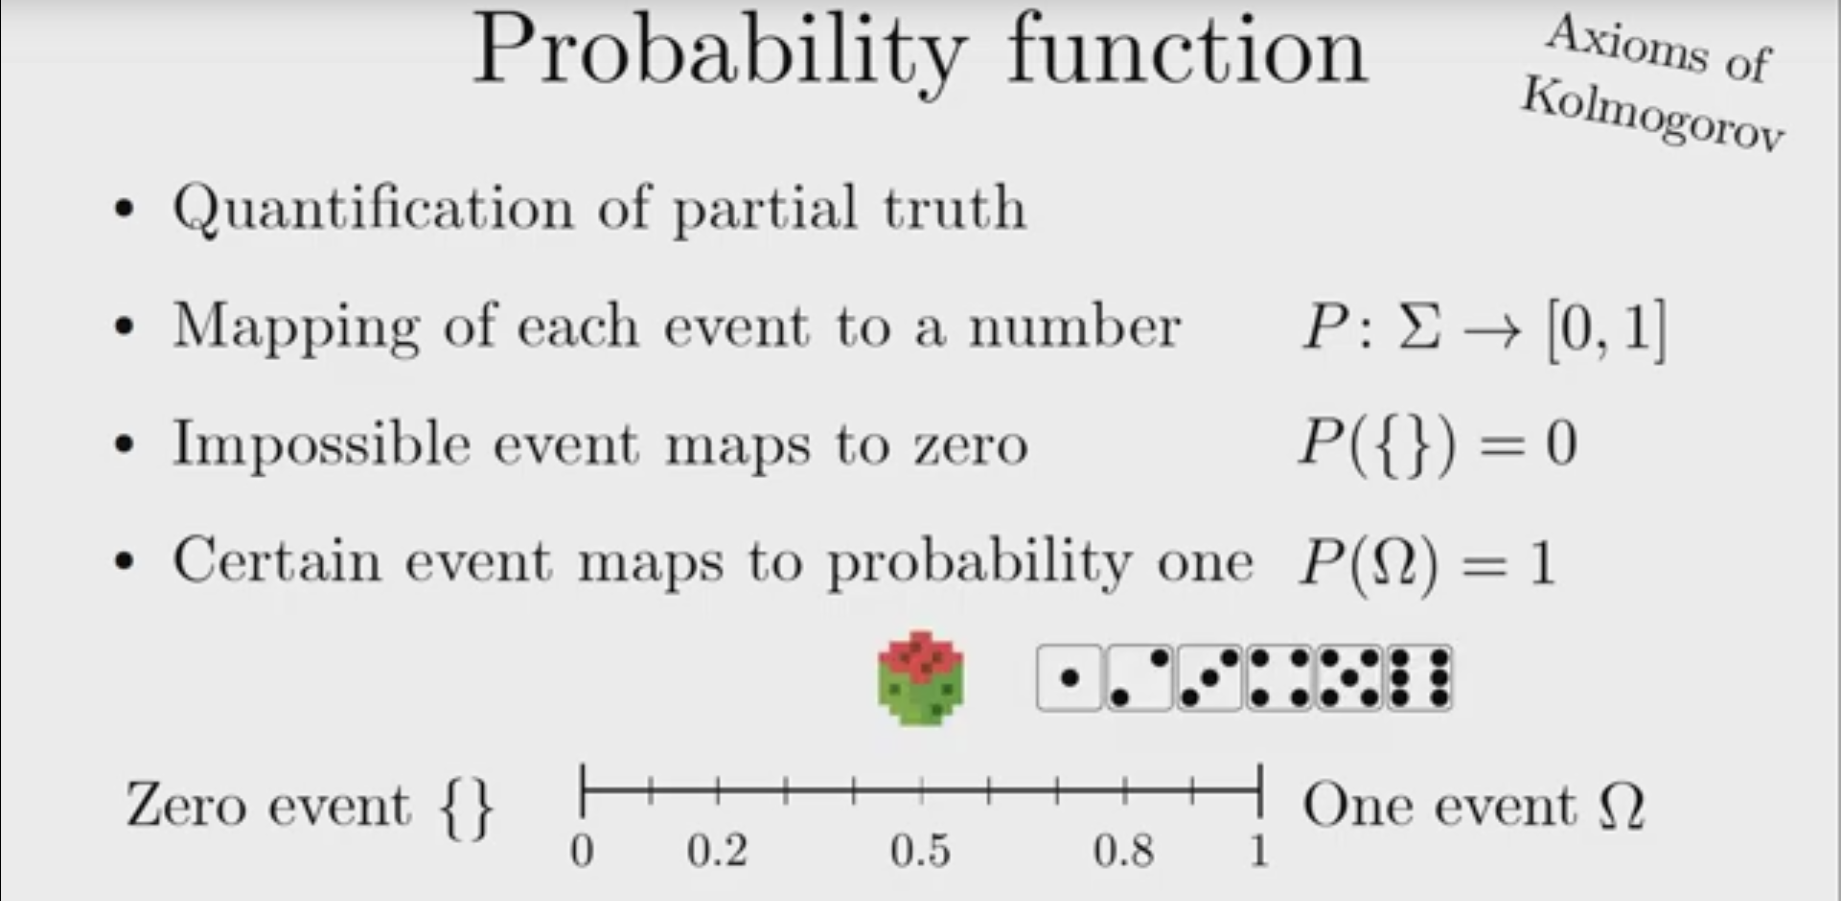
\includegraphics[width=0.75\textwidth]{1_2.png}
\end{figure}
To be able to work with probabilities we need the rules of probability theory. There are two basic rules in probability theory, which can be explained most easily by set algebra.
Since events are sets, we will use \textbf{Venn diagrams} to illustrate them.
A set, or a subset, is depicted by ellipses. Since each event is a subset of the sample space $\Omega$ it can be drawn as an ellipse inside $\Omega$. The first rule of probability theory concerns the logical or of two events A and B say, which corresponds to the union of two subsets. The probability for A or B is treated in the \textbf{sum rule}. To begin with, we consider exclusive events A and B, which have no overlap. For those, the sum rule states, that the probability for A or B is the sum of the individual probabilities. It is particularly obvious if we identify the probabilities with the area of the ellipses. In that case the union of the two sets is equal to the sum of both areas.
A special case applies to the \textbf{complement} of the set A, or the corresponding event, and can be depicted as the area inside $\Omega$, that is NOT A.
In this case the sample space $\Omega$ contains both, A and NOT A. Remember, that we have defined the probability of the sample space $\Omega$ to be equal to one. Therefore, we get for the probability of the complement of an event: one minus the probability of that event.
For non-exclusive events there might be an overlap which corresponds to the intersection of two sets. If we sum the probabilities for the events A and B. We count the elements contained in the intersection of the sets A and B twice. Therefore, we have to subtract the probability for the event (A and B). That brings us to the generally valid form of the sum rule. 
\fbox{\parbox{\linewidth}{
\begin{centering}
\textbf{Sum rule}
\[P(A \cup B) = P(A) + P(B) - P(A \cap B)\]
\end{centering}
}}
\\
\begin{figure}[H]
	\centering
	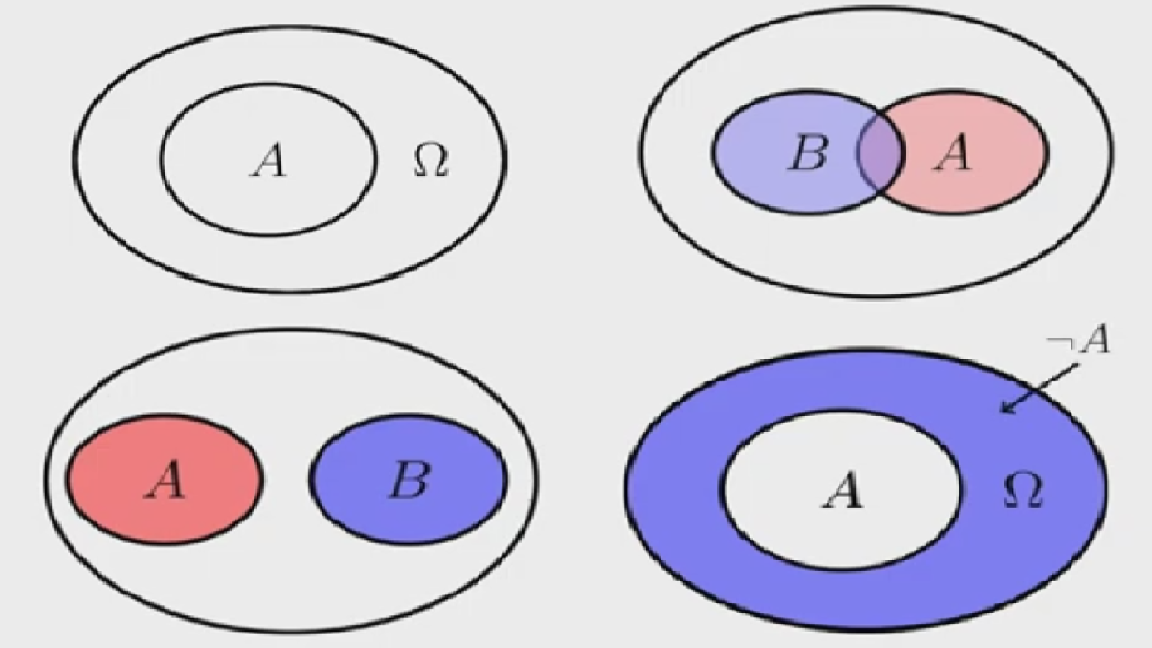
\includegraphics[width=0.75\textwidth]{1_3.png}
\end{figure}

The second rule of probability theory, the so called \textbf{product rule}, tells us how to work with events that are combined by the logical AND. Like the term that we subtracted in the sum rule. A detailed discussion of the product rule follows in unit three. There are now some questions for you to train these concepts.\\

\fbox{\parbox{\linewidth}{\textbf{Question 4.} What is the probability that your birthday falls on the weekend?\\
a) 1/7 + 1/7\\
b) It's not possible to answer this question.\\
c) P(your birthday is on Saturday) + P(your birthday is on Sunday)\\
\textbf{Question 5.} What is the probability that my birthday (B) is not on a Friday (we use the notation: ``B is on X'' means ``my birthday is on x''?\\
a) P(B is on Monday) + P(B is on Tuesday) + P(B is on Wednesday) + P(B is on Thursday) + P(B is on Saturday) + P(B is on Sunday)\\
b) P(B is on Friday)\\
c) 1 - P(B is on Friday)\\
d) 6/7\\
\textbf{Question 6.} What is the probability that my birthday (B) is not on a Friday (we use the notation: ``B is on X'' means ``my birthday is on x''?\\
a) P(B is on Monday) + P(B is on Tuesday) + P(B is on Wednesday) + P(B is on Thursday) + P(B is on Saturday) + P(B is on Sunday)\\
b) P(B is on Friday)\\
c) 1 - P(B is on Friday)\\
d) 6/7
\textbf{Question 7.} What is the sum rule for having an odd number of pips or a prime number of pips when rolling a dice?\\
a) P(odd) + P(prime) - P(odd or prime)\\
b) P(odd) + P(prime)\\
c) P(odd) + P(prime) - P(odd and prime)\\
d) P(\{1,3,5\}) + P(\{2, 3, 5\}) - P(\{3, 5\})
}}
\\

There is also an alternative way to express probability, which is called \textbf{odds}. 
Odds map events not to the interval zero to one but to any positive number and they are commonly used in sport bets and some applications of statistics.
The odds of an event A can be directly calculated from its probability by the ratio of P for A divided by the probability for its negation (P for not A). 
Odds represent the chance that an event will occur, compared to the chances, that the opposite will happen. For example: the Odds of two to three for an event states that on average you can expect two times the desired event and three times its negation, which corresponds to a probability of two divided by five or zero point four.
In many cases a colon  (:) is used to distinguish odds from probabilities.
Note however, that the sum rule and product rule do not apply to odds. Nevertheless, odds will become useful in a later chapter when we discuss Bayesian update rules of knowledge. \\

\fbox{\parbox{\linewidth}{
\textbf{Question 8.} Order the correct values to complete the text: ``2 to 3'', ``12.5\%'', ``1 to 3'', ``3 to 3''\\
a) are the offs for a probability of 25\%.\\
b) are the offs for a probability of 2/5.\\
c) is the probability for odds of 1:7.\\
d) are the offs for a probability of 1/2.
}}
\\

Now, that we have learned Kolmogorov’s axioms and the rules of how to work with probabilities the next question is how to assign probabilities, how to get the values.
There are actually three ways to do so. First, we will discuss the \textbf{classical approach}, which works in the case when elementary events are assumed to be equally probable. Although it seems like a circular argument there are many examples where it works very successfully.
The other two alternative approaches will be discussed in future units and I will introduce them here, just as an outlook. The \textbf{frequentist approach} is based on statistics and defines probabilities as relative frequencies of measured data. This is sometimes called \textbf{orthodox statistics}.
The \textbf{Bayesian approach} is the main focus of this course. Here, probability has a very general meaning. For the assignment for probabilities, we will discuss the principle of transformation groups to deal with continuous variables to assign probabilities for events if nothing is known apart from their definition. You will also learn the \textbf{principle of maximum entropy}. That allows you to assign probabilities based on additional knowledge. In this context we will rediscover some results of the classical approach as special cases. \\

Now let’s see how our friends Bernoulli and Laplace solved probabilistic problems in the classical way. %%
\begin{figure}[H]
	\centering
	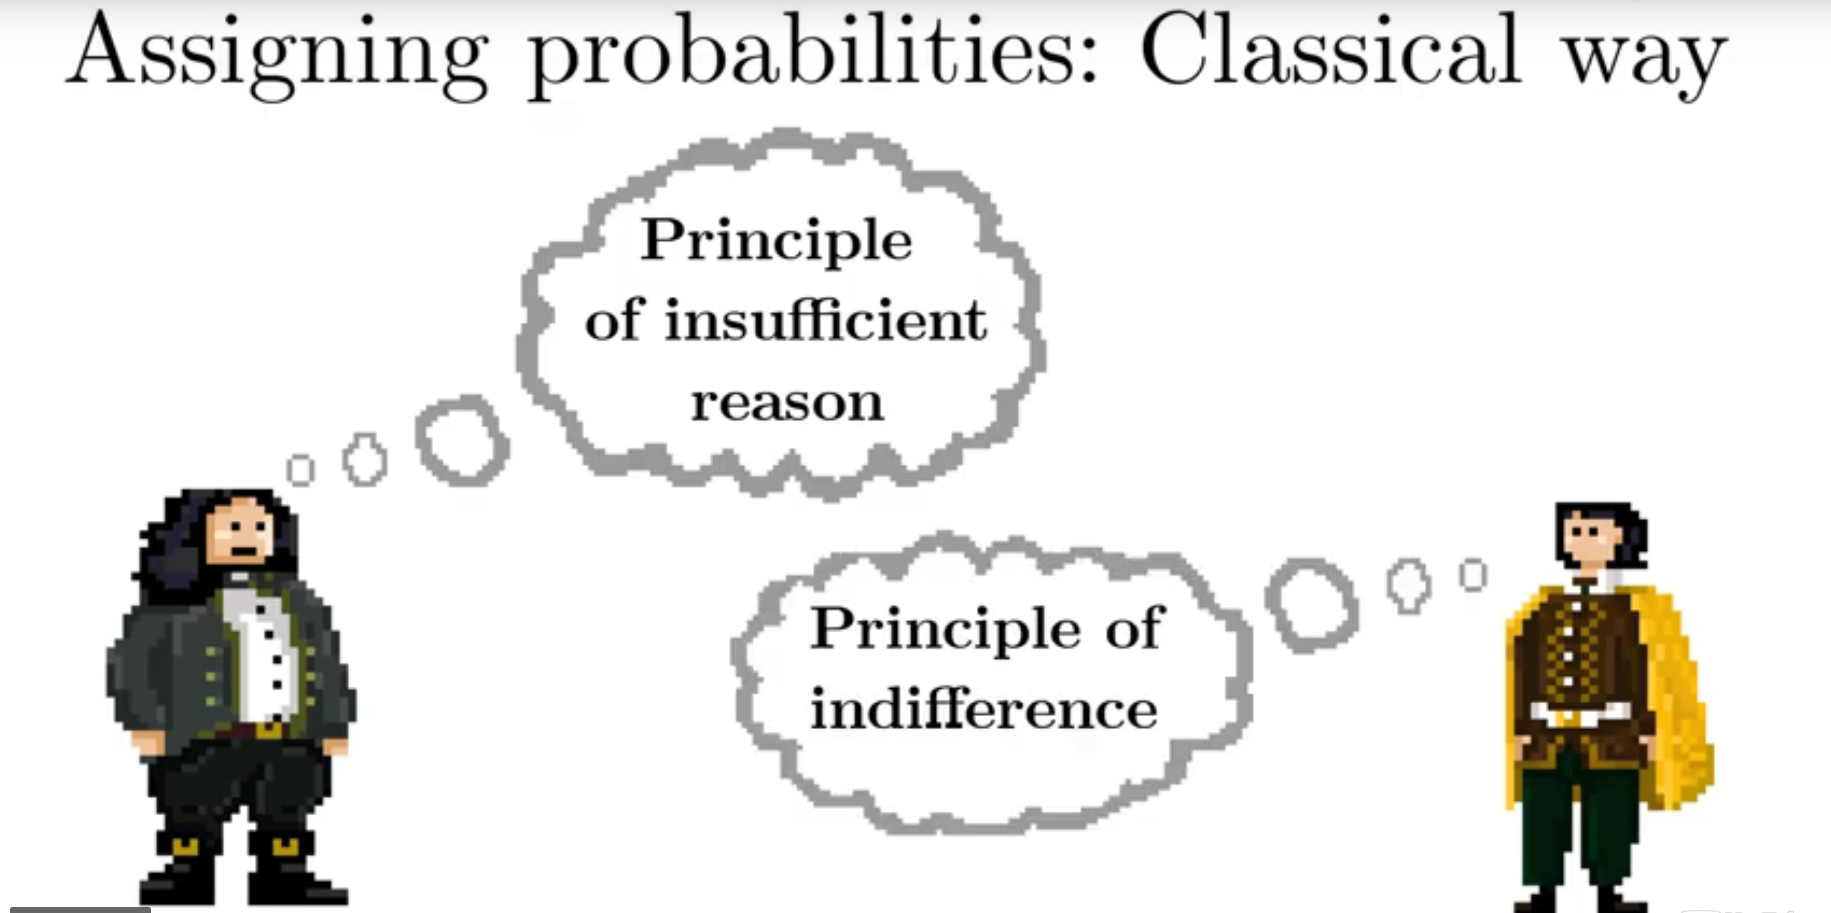
\includegraphics[width=0.75\textwidth]{1_4.png}
\end{figure}
They formulated the \textbf{principle of insufficient reason}, also known as the \textbf{principle of indifference}, which states the following:\\
\fbox{\parbox{\linewidth}{
\begin{centering}
\textit{If the elementary events – the outcomes – of an experiment can be regarded as equal in the sense that none of them is preferred in any way, then we can assign the same probability to all of them.}\\
\end{centering} }}
This is often true in the case of symmetric objects, like a dice or a disk as we have seen with the random compass, and it can also be due to missing information.
For a perfectly symmetric dice with six outcomes this leads to an equal probability for each of the six outcomes of one sixth, or which is approx. 17\%. 
For the coin, the probability for each side is one half.\\

Next, we want to generalize these ideas to general events. For the case of equally probable elementary events, the classical definition of probabilities of general events is given by the ratio of the number of \textbf{favorable outcomes} to the number of \textbf{possible outcomes}. This follows readily from the sum rule of exclusive events. %
Let’s consider the dice again as example: For the event of an odd number of pips on a dice there are three outcomes that make the event true: one, three and five.
\begin{figure}[H]
	\centering
	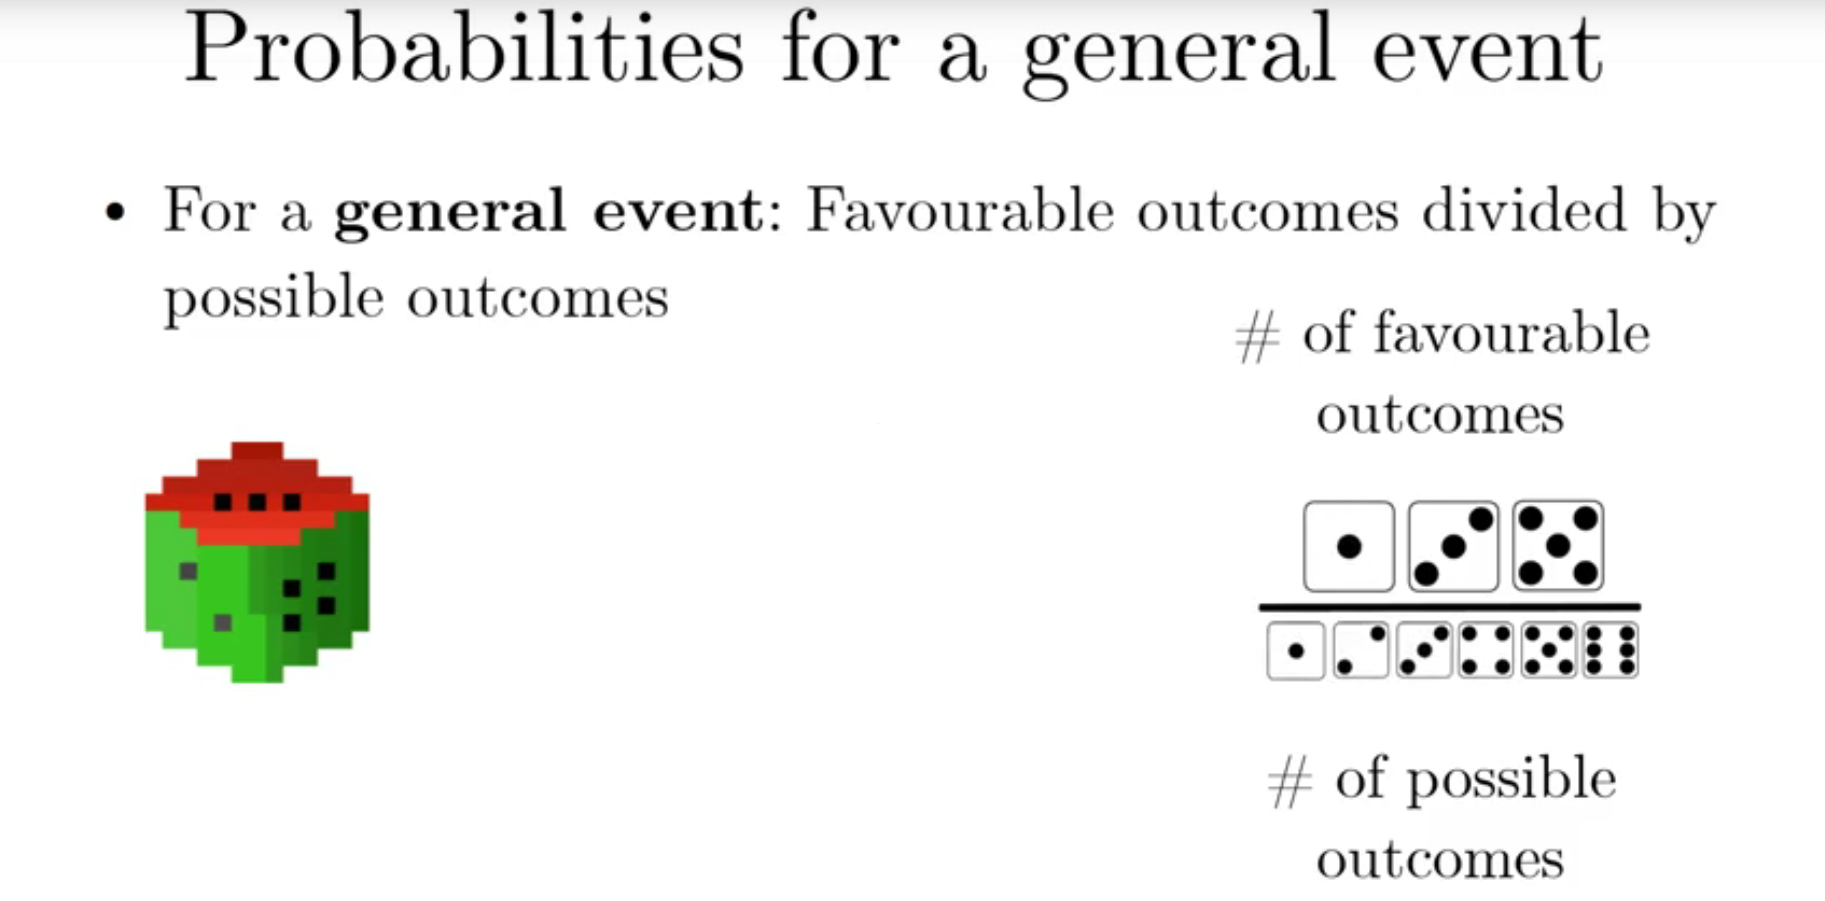
\includegraphics[width=0.75\textwidth]{1_5.png}
\end{figure}
The total number of outcomes is six, so the probability of the event of having an odd number of pips on a dice is three divided by six which is one half. Here we could also argue with the principle of indifference. Three sides show an even number of pips and three sides an odd number. There is no way we can distinguish these two sets of sides. Therefore, odds and even numbers of pips should have the same probability, namely 0.5.\\

\fbox{\parbox{\linewidth}{
\textbf{Question 9.} Complete the text: ``due to performing lots of experiments/experience'', ``the perfect symmetric shape'', ``new information''\\
We know that the probability for 6 pips on a dice is due to .......... \\
Laplace Might be able to quantify the probability for having roast for dinner due to .............. \\
Bernulli knows the probability for sailing deviations ..........
}}
\\

The question of the probability of having a day off on Captain Bayes’s ship is trickier. First, one has to identify the full sample space $\Omega$. Since the compass needle is twisted twice, one has to combine each result of the first dial with all four possible results of the second dial, resulting in a total of 16 possible outcomes.
Now, the order of directions is important. North-West is a different outcome than West-North. In contrast to the curly brackets for sets we now use round brackets for these tuples to indicate that the sequence is important.
In the second step we need to identify the favorable outcomes for the "Free day" event, namely North-South, South-North, East-West and West-East. Hence, there are four favorable outcomes.
The probability for the free day event is thus given by four divided by 16, which is equal to 25 \%.\\
\begin{figure}[H]
	\centering
	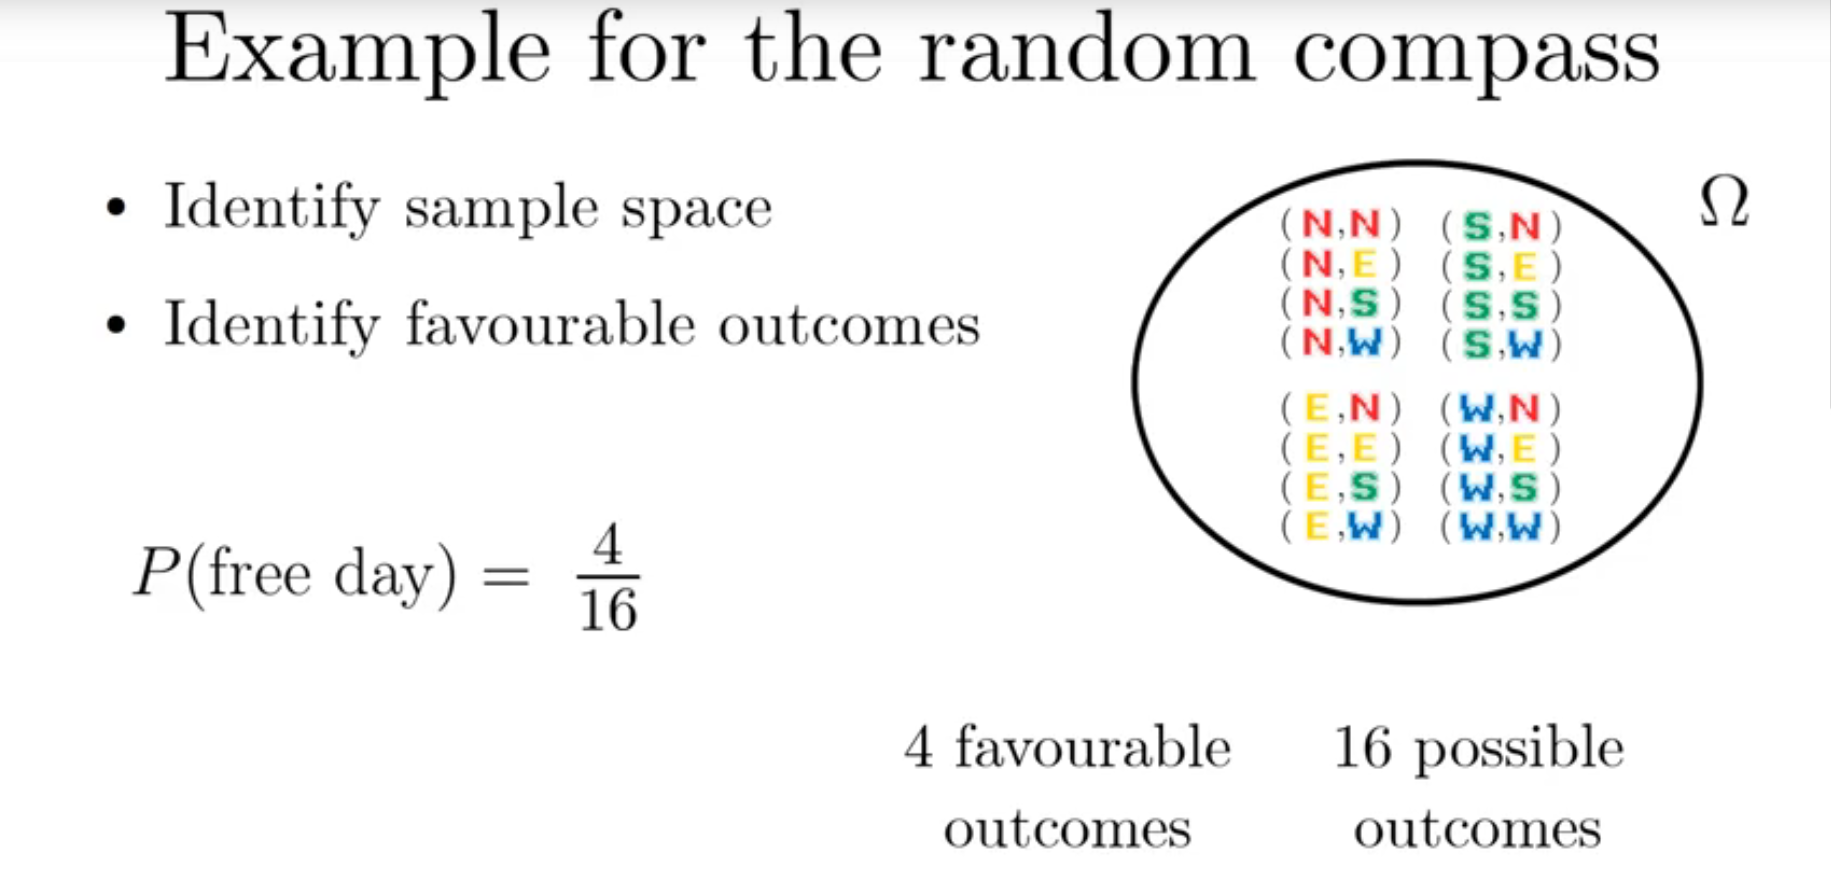
\includegraphics[width=0.75\textwidth]{1_6.png}
\end{figure}
\fbox{\parbox{\linewidth}{
\textbf{Question 10.} What is the probability of having at least once East or West when dialing twice?\\
a) 50\%\\
b) 75\%\\
c) 40\%\\
d)12/16\\
e) 25\%
}}
\\

This concludes the first unit. Please have a look at the bonus material, feel free to ask questions in our forum and be encouraged to test your knowledge in the quiz.\\


\end{document}